\documentclass[a4paper]{extarticle}
\usepackage[utf8]{inputenc}
\usepackage[a4paper, margin=1in]{geometry}

\usepackage{amssymb}
\usepackage{amsmath}
\usepackage{enumitem}
\usepackage{tcolorbox}
\usepackage{fancyhdr}
\usepackage{graphicx}
\usepackage{float}

\setlength{\parindent}{0em}
\setlength{\parskip}{0.4em}

\definecolor{theoremblue}{RGB}{1, 73, 124}
\definecolor{corollaryblue}{RGB}{70, 143, 175}
\definecolor{exampleblue}{RGB}{137, 194, 217}

\newtcolorbox{tbox}{colback=theoremblue!20,colframe=theoremblue,
boxrule=0pt,arc=0pt,boxsep=2pt,left=2pt,right=2pt,leftrule=2pt}

\newtcolorbox{cbox}{colback=corollaryblue!20,colframe=corollaryblue,
boxrule=0pt,arc=0pt,boxsep=2pt,left=2pt,right=2pt,leftrule=2pt}

\newtcolorbox{ebox}{colback=exampleblue!20,colframe=exampleblue,
boxrule=0pt,arc=0pt,boxsep=2pt,left=2pt,right=2pt,leftrule=2pt}

\title{IntroML - Lecture Notes Week 10}
\author{Ruben Schenk, ruben.schenk@inf.ethz.ch}
\date{\today}

\pagestyle{fancy}
\fancyhf{}
\rhead{ruben.schenk@inf.ethz.ch}
\rfoot{Page \thepage}
\lhead{IntroML - Lecture Notes Week 10}

\begin{document}

\maketitle

\section{Statistical Perspective on Supervised Learning}

\subsection{Introduction}

We have seen how we can fit prediction models for regression and classification. We will now explore a \textbf{statistical perspective} on supervised learning, i.e. estimate the data distribution and derive some prediction/decision rule from the distribution.

Benefits are:
\begin{itemize}
    \item Quantify the uncertainty
    \item Express prio knowledge/assumptions about the data
    \item Allows to derive new methods
\end{itemize}

Recall the general goal of supervised learning: Given the training data $D = \{(x_1, \, y_i),..., \, (x_n, \, y_n)\} \subseteq X \times Y$. We want to identify a hypothesis $f : X \to Y$ from some class $F$, e.g.:
\begin{itemize}
    \item Linear models: $f(x) = w^Tx$
    \item Kernel methods: $f(x) = \sum_i \alpha_i k(x_i, \, x)$
    \item Neural networks: $f(x) \sum_i w_i' \sigma(w_i^T x)$
\end{itemize}
Our goal is to minimize the prediction error, i.e. the loss on unseen examples. But what does this mean more formally? When can we hope that learning will succeed?

The fundamental assumption is that our data set is generated independently and identically distributed (i.i.d.), i.e.
\[
    (x_i, \, y_i) \sim p(x, \, y)
\]
for some unknown $p$. We would like to identify a hypothesis $f: X \to Y$ that minimizes the expected loss (prediction error, population risk):
\[
    R(f) = \int p(x, \, y)l(y; \, f(x)) \, dxdy = \mathbb{E}_{x, \, y}[l(y; \, f(x))].
\]

\subsection{Estimating Generalized Error}

We can estimate the generalized error by estimating the true risk by the empirical risk on the sample data set $D$ (\textit{Empirical Risk Minimization (ERM)}):
\[
    \hat{R}_D(f) = \frac{1}{|D|}\sum_{(x, \, y) \in D} l(y; \, f(x)).
\]
Why might this work? Because of the law of large numbers (LLN): $\hat{R}_D(f) \to R(f)$ almost surely as $|D| \to \infty$.

\begin{figure}[H]
    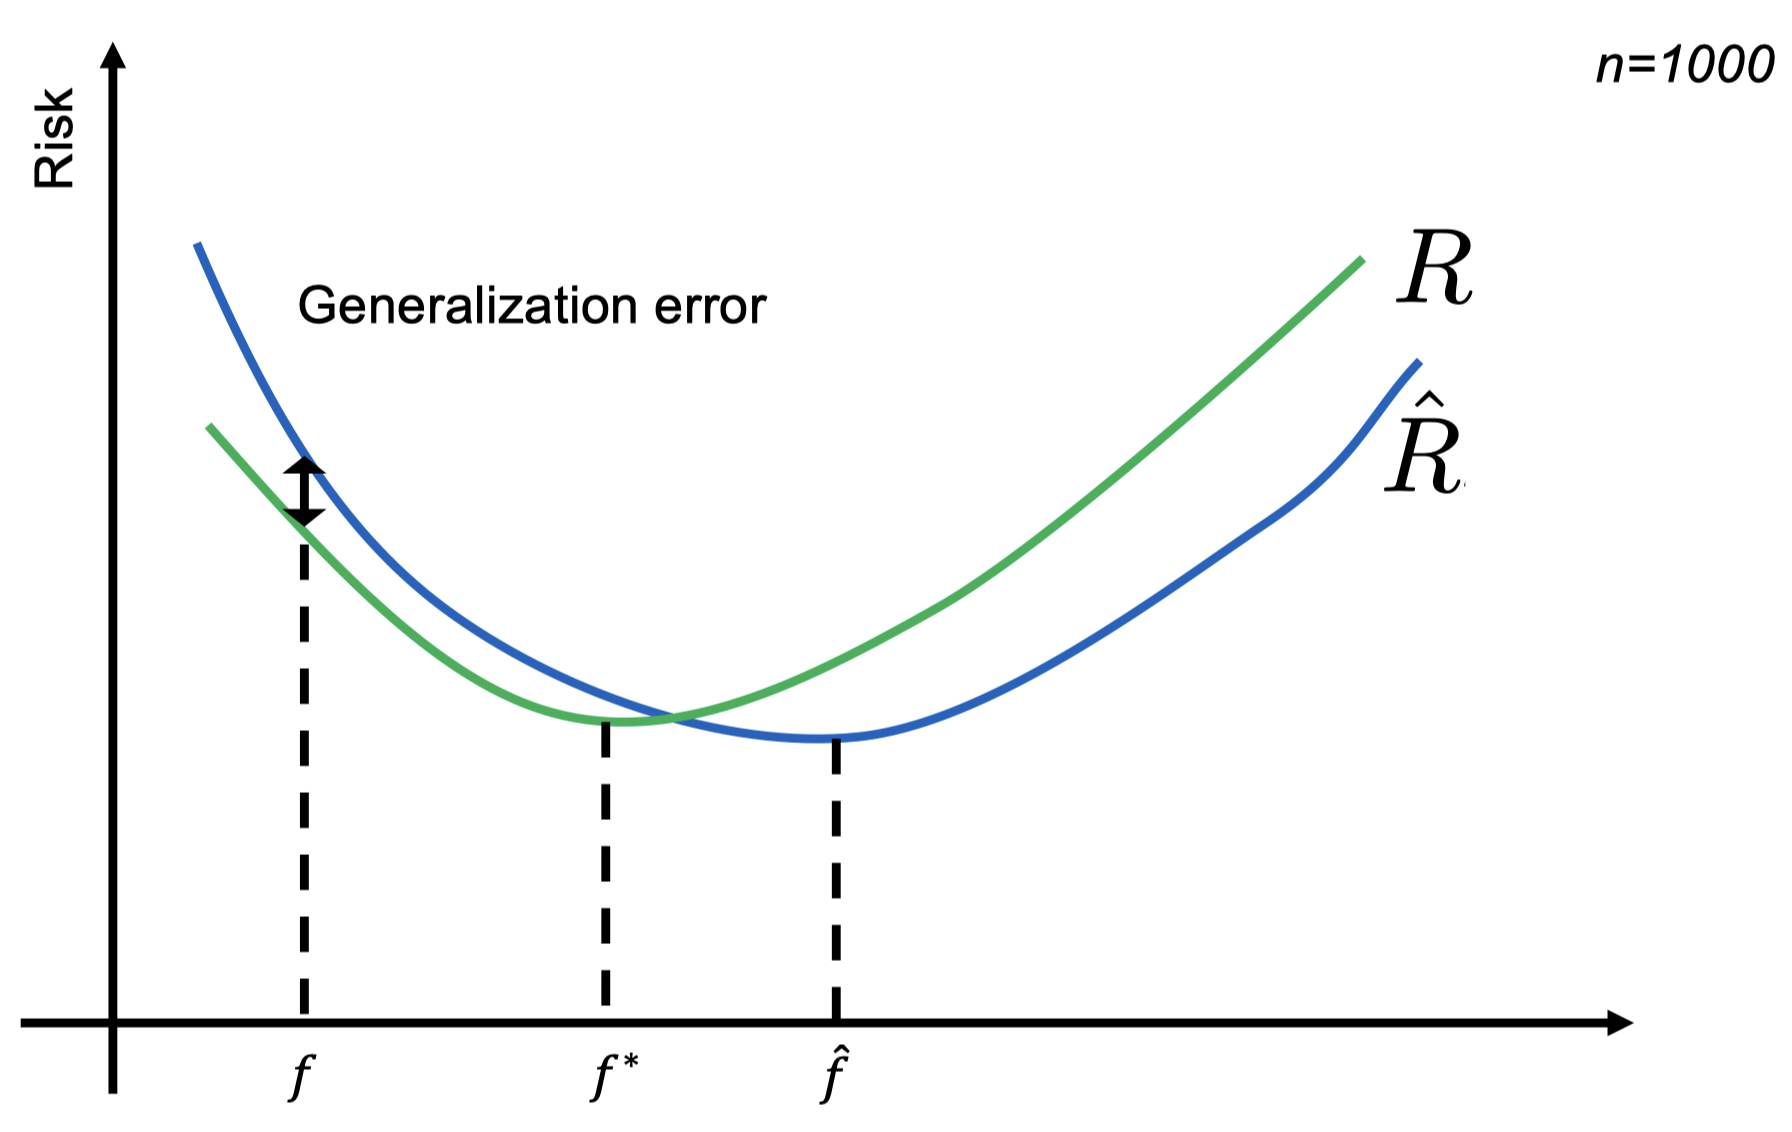
\includegraphics[width=9cm]{../images/IntroML_Fig10-1}
    \centering
\end{figure}

The more samples you take (higher $n$), the closer the two curves go together!

What happens if we optimize on training data? Assume we are given training data $D$ and obtain some solution $\hat{f}_D = \arg \min_{f \in F} \hat{R}_D(f)$. Ideally, we wish to solve for $f^* = \arg \min_{f \in F}R(f)$. However, in general, it will hold that $\mathbb{E}_D[\hat{R}_D(\hat{f}_D)] \leq \mathbb{E}_D[R(\hat{f}_D)]$. Thus, we obtain an \textit{overly optimistic estimate.}

What would be a more realistic evaluation? We want to avoid underestimating the prediction error. The idea is as follows: We obtain training ($D$) and test data ($D'$) from the same distribution $p$. Then we optimize $f$ on the training set, i.e. $\hat{f}_D = \arg \min_{f \in F} \hat{R}_D(f)$. We evaluate on the test set
\[
    \hat{R}_{D'}(\hat{f}_D) = \frac{1}{|D'|}\sum_{(x, \, y) \in D'}l(y; \, \hat{f}_D(x)).
\]
Then it holds that:
\[
    \mathbb{E}_D'[\hat{R}_{D'}(\hat{f}_D)] = R(\hat{f}_D)
\]

The i.i.d. assumption is a standard assumption, but often violated in practice! E.g. temporal dependencies, spatial/geographic dependencies, sampling bias, strategic behavior, etc.

\subsection{Optimal Predictor for Squared Loss}

For the squared loss, the population risk is
\[
    R(f) = \mathbb{E}_{x, \, y}[(y - f(x))^2].
\]
Suppose we (unrealistically) knew $p(x, \, y)$, and we allow arbitrary functions $f$. Which $f$ minimizes the risk?

Assuming the data is generated i.i.d. according to $(x_i, \, y_i) \sim p(x, \, y)$. The hypothesis $f^*$ minimizing $R(f)$ is given by the \textbf{conditional mean:}
\[
    f^*(x) = \mathbb{E}[Y \, | \, X = x]
\]
This (in practice unattainable) hypothesis is called the \textbf{Baye's optimal predictor} for the squared loss.
\textbf{Note:} We only need the conditional distribution $p(y \, | \, x)$. not the full joint distribution $p(x, \, y)$.

In practice, we have finite data. We know that $f^*(x) = \mathbb{E}[Y \, | \, X = x]$. Thus, one strategy for estimating a predictor from training data is to estimate the conditional distribution $\hat{p}(y \, | \, x)$ and then, for some test point $x$, predict the label via the conditional mean:
\[
    \hat{y} = \hat{\mathbb{E}}[Y \, | \, X = x] := \int y \hat{p}(y \, | \, x) \, dy
\]

The common approach for estimating conditional distributions is by \textbf{parametric estimation} $\hat{p}(y \, | \, x, \, \theta)$:
\begin{enumerate}
    \item Choose a particular parametric form
    \item Then estimate the parameters $\theta$
\end{enumerate}
Step 2 is done using maximum (conditional) Likelihood estimation:
\[
    \theta^* = \arg \max_{\theta} \hat{p}(y_1,..., \, y_n \, | \, x_1,..., \, x_n, \, \theta)
\]

\subsection{Probabilistic Model for Regression}

Consider linear regression. Let's make the statistical assumption that the noise is Gaussian, i.e.:
\[
    y_i = w^Tx_i + \epsilon_i \text{ where } \epsilon_i \sim \mathcal{N}(0, \, \sigma^2)
\]
Then we can compute the conditional likelihood of the data given any candidate model $w$ as:
\[
    \hat{w} = \arg \min_{w} \sum_{i = 1}^n (y_i - w^Tx_i)^2
\]
thus, under the "conditional linear Gaussian" assumption, maximizing the likelihood is equivalent to least squares estimation.

This observation is actuall not tied to linear models. Suppose $F = \{f : X \to \mathbb{R}\}$ is a class of functions. Assuming that $p(Y = y \, | \, X = x) = \mathcal{N}(y \, | \, f^*(x), \ \sigma^2)$ for some function $f^* : X \to Y$ in $F$ and some $\sigma^2 > 0$, the MLE for data $D = \{(x_1, \, y_1),..., \, (x_n, \, y_n)\}$ is given by
\[
    \hat{f} = \arg \min_{f \in F} \sum_{i = 1}^n (y_i - f(x_i))^2.
\]

In summary, the maximum likelihood estimate (MLE) is given by the least squares solution, assuming that the noise is i.i.d. Gaussianm with constant variance. This is useful since MLE satisfies several nice statistical properties (not fromally defined here):
\begin{enumerate}
    \item Consistency: parameter estimate converges to true parameters in probability
    \item Asymptotic efficiency: smallest variance among all "well-behaved" estimators for large $n$
    \item Asymptotic normality
\end{enumerate}
\textit{However,} all these properties are asymptotic (hold as $n \to \infty$). For finite $n$, we must avoid overfitting!

\subsection{Bias, Variance, and Noise}

Recall the \textbf{bias variance tradeoff:}
\[
    \text{Prediction error} = \text{Bias}^2 + \text{Variance} + \text{Noise}
\]
\begin{itemize}
    \item Bias: Excess risk of best model considered compared to minimal achievable risk knowing $p(x, \, y)$ (i.e. given infinite data)
    \item Variance: Risk incurred due to estimating model from limited data
    \item Noise: Risk incurred by optimal model (i.e. irreducible error)
\end{itemize}

\subsubsection{Bias in Estimation}

MLE solution depends on training data $D$. But the training data $D$ is itself random, i.e. drawn i.i.d. from $p$. We might want to choose $F$ to have small \textbf{bias,} i.e. to have a small squared error on average:

\[
    \mathbb{E}_x[\bar{f}(x) - f^*(x)]^2 \text{ for } \bar{f}(x) := \mathbb{E}_D[\hat{f}_D(x)].
\]

\begin{figure}[H]
    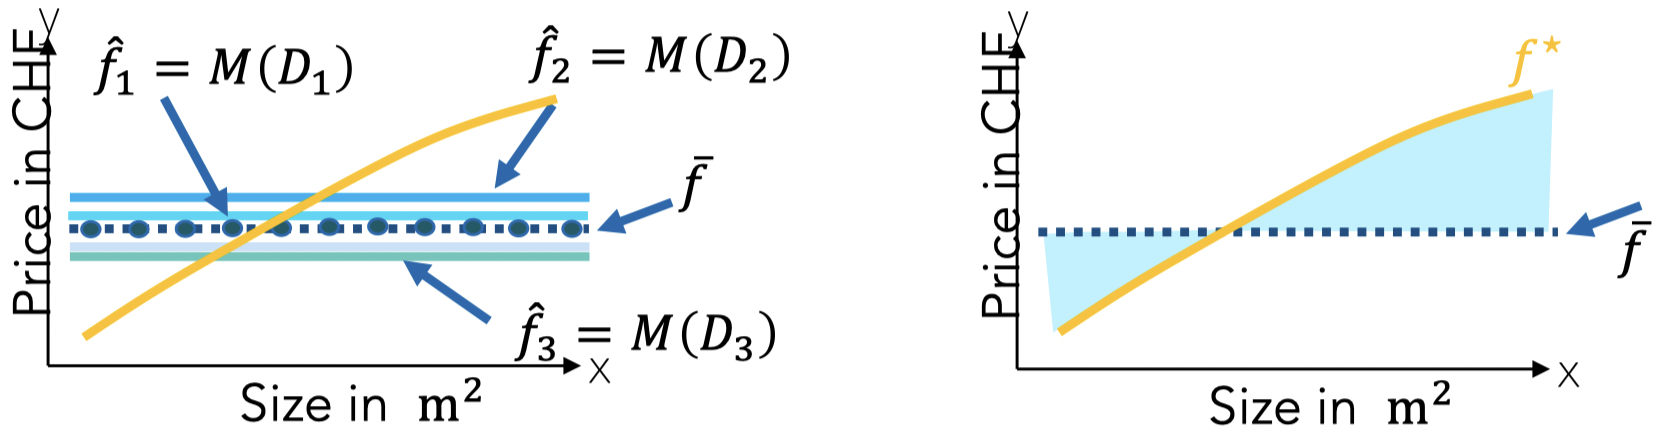
\includegraphics[width=15cm]{../images/IntroML_Fig10-2}
    \centering
\end{figure}

\subsubsection{Variance in Estimation}

The estimator MLE is itself random, and has some variance:

\[
    \mathbb{E}_x[\text{Var}_D[\hat{f}_D(x)]] = \mathbb{E}_x[\mathbb{E}_D[(\hat{f}_D(x) - \bar{f}(x))^2]]
\]

\begin{figure}[H]
    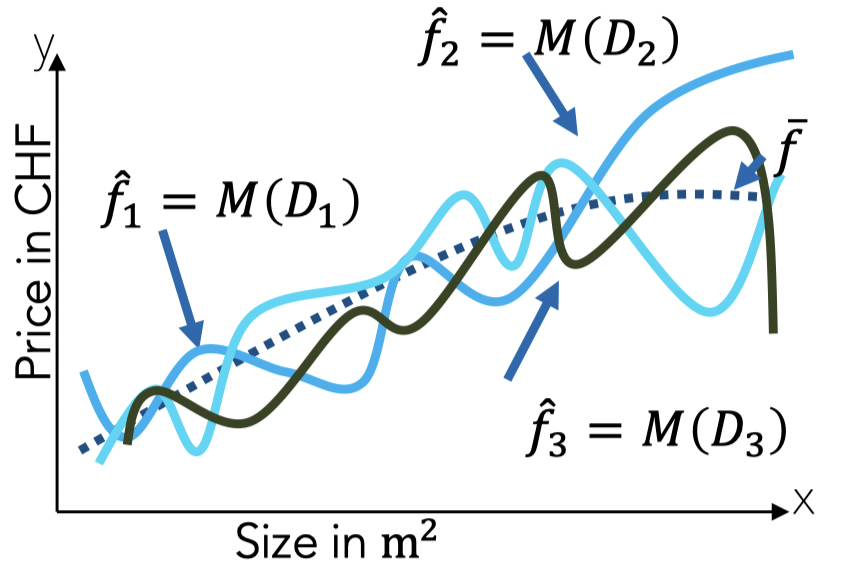
\includegraphics[width=8cm]{../images/IntroML_Fig10-3}
    \centering
\end{figure}

\subsubsection{Noise in Estimation}

Even if we know the Bayes' optimal hypothesis $f^*$, we'd still incur some error due to noise:
\[
    \mathbb{E}_{x, \, y}[(y - f^*(x))^2]
\]
This error is \textit{irreducible,} i.e. independent of choice of the hypothesis class.

\subsubsection{Bias-Variance Tradeoff}

For least-squares estimation the following holds:
\[
    \mathbb{E}_{D, \, x, \, y}[(y - \hat{f}_D(x))^2] = \mathbb{E}_x[\bar{f}(x) - f^*(x)]^2 + \mathbb{E}_x[\text{Var}_D[\hat{f}_D(x)]] + \mathbb{E}_{x, \, y}[y - f^*(x)]^2,
\]
\[
    \text{Expected Mean Squared Prediction Error} = \text{Bias}^2 + \text{Variance} + \text{Noise},
\]
where $\hat{f}(x) = \mathbb{E}_D[\hat{f}_D(x)]$ and $\text{Var}_D[\hat{f}_D(x)] = \mathbb{E}_D[(\hat{f}_D(x) - \bar{f}(x))^2]$.
Ideally, we wish to find an estimator that simultaneously minimizes bias and variance.

\begin{figure}[H]
    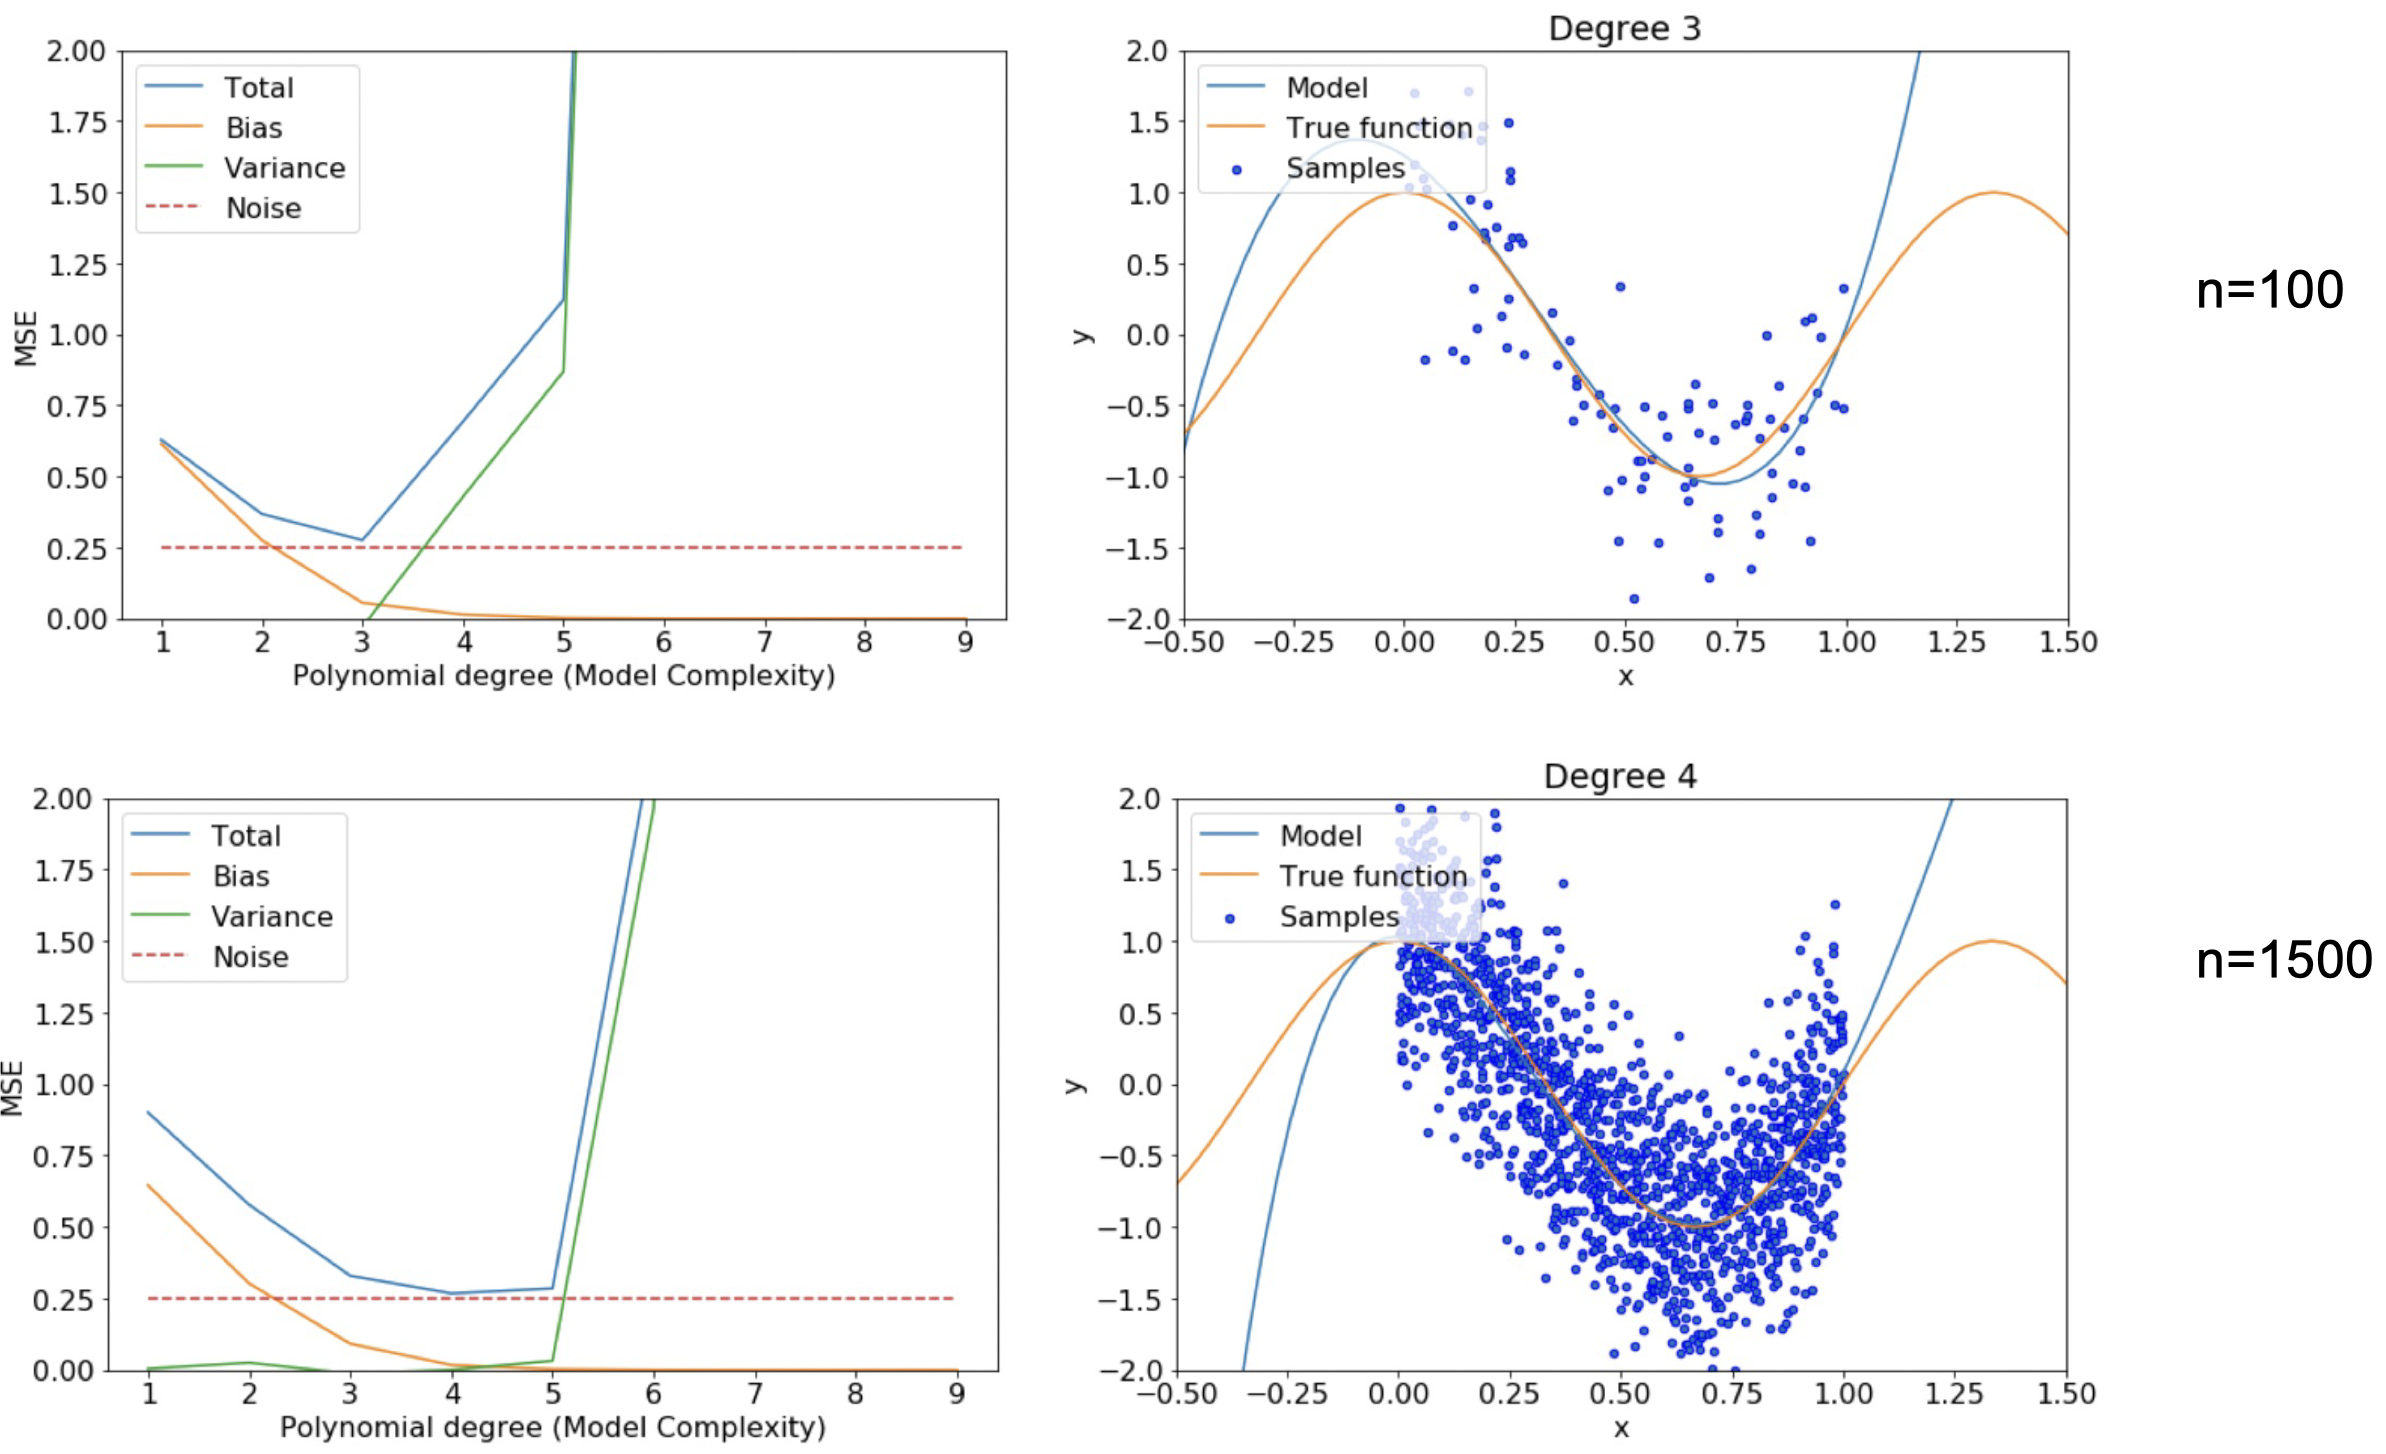
\includegraphics[width=15cm]{../images/IntroML_Fig10-4}
    \centering
\end{figure}

The maximum likelihood estimate for linear regression is unbiased (if $f^* \in F$). Furthermore, it is the maximum variance estimator among all unbiased estimators. However, we have already seen that the least-squares solution can overfit.
Thus, we might trade a little bit of bias for a (potentially dramatic) reduction in variance.

\end{document}